%% LyX 2.2.3 created this file.  For more info, see http://www.lyx.org/.
%% Do not edit unless you really know what you are doing.
\documentclass[english]{article}
\usepackage[T1]{fontenc}
\usepackage[utf8]{inputenc}
\usepackage{geometry}
\geometry{verbose,rmargin=3cm,bmargin=2cm, footskip=1cm, tmargin=2cm}
\usepackage{float}
\usepackage{textcomp}
\usepackage{graphicx}
\usepackage{verbatim}
\usepackage{amsmath}
\usepackage{hyperref}
\hypersetup{colorlinks=true}
\usepackage{color}
\definecolor{myred}{rgb}{1,0.98,0.98}
\makeatletter

%%%%%%%%%%%%%%%%%%%%%%%%%%%%%% LyX specific LaTeX commands.
%% Because html converters don't know tabularnewline
\providecommand{\tabularnewline}{\\}

\@ifundefined{date}{}{\date{}}
%%%%%%%%%%%%%%%%%%%%%%%%%%%%%% User specified LaTeX commands.

\usepackage{array}
\usepackage{color}
\usepackage{colortbl}

\makeatother

\usepackage{babel}
\usepackage{listings}
\renewcommand{\lstlistingname}{Listing}

\title{Tutorato Architettura degli Elaboratori Modulo 2 \\ Lezione 3}
\author{Francesco Pelosin}
\date{18 Aprile 2019}

\begin{document}
\lstset{frame=single, numbers=left, backgroundcolor=\color{myred}}
\maketitle

\section{Gerarchie di Memoria}

\begin{figure}[H]
    \centering
    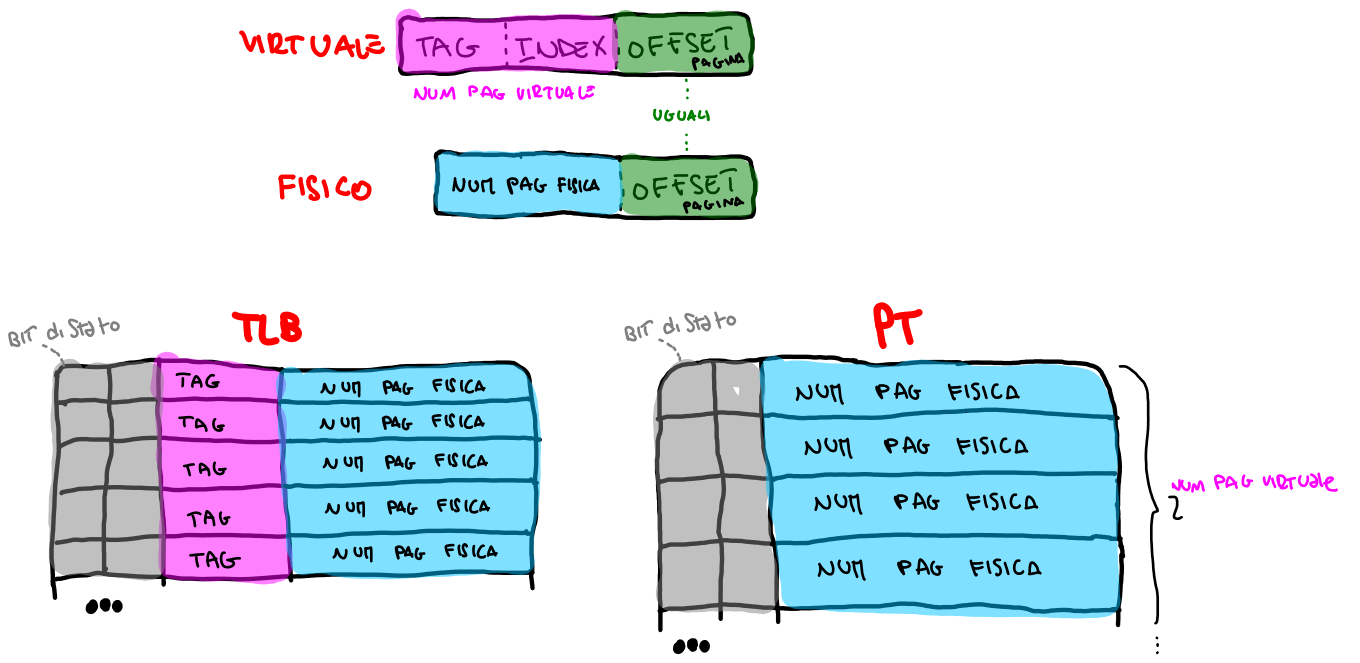
\includegraphics[width=1\textwidth]{gerarchia.png}
    \caption{Remainder organizzazione.}
\end{figure}

%%%%%%%%%%%%%%%%%%%%%%%%%%%%%%%%%%%%%%%%%%%%%%%%%%%%%%%%%%%%%%%
\subsection*{Esercizio 1}
%%%%%%%%%%%%%%%%%%%%%%%%%%%%%%%%%%%%%%%%%%%%%%%%%%%%%%%%%%%%%%%
Si consideri un sistema di memoria virtuale paginata con indirizzo virtuale di 32 b e indirizzo fisico di 27 b. Il sistema comprende una TLB 4-way associative, con 512 ingressi totali (blocchi), e \texttt{TAG} di 13 b. Calcolare la $PageSize$ (1). 
Infine, la cache del sistema è 8-way associative, la parte dati è 1 MB, e il $BlockSize$ è di 16 B. Calcolare \texttt{TAG} e l'\texttt{INDEX} (2).

% -.-.-.-.-.-.-.-.-.-.-.-.-.-.-.-.-.-.-.-.-.-.-.-.-.-.-.-.-.-.-
\subsubsection*{Soluzione}
% -.-.-.-.-.-.-.-.-.-.-.-.-.-.-.-.-.-.-.-.-.-.-.-.-.-.-.-.-.-.-


\begin{enumerate}
    \item Essendo la TLB una 4-way associative abbiamo che $\#linee = 512/4 = 128 = 2^{7}$, di conseguenza sappiamo che per indicizzare la TLB occorrono 7 bit che andremo a prendere dall'indirizzo virtuale. Avremmo quindi che la quantità di bit di \texttt{OFFSET} dell'indirizzo virtuale sarà: 32-13-7 = 12. Con 12 bit possiamo dunque indicizzare $2^{12}$ Byte di conseguenza la $PageSize$ sarà 4KB.
    
    \item Per calcolare l'\texttt{INDEX} dobbiamo sapere il numero di linee ($\#linee$) della cache. Per fare questo prima dobbiamo ricavare $\#blocchi = 1MB / 16 B = 2^{23} / 2^{7} = 2^{16}$. Ora possiamo ricavare $\#linee$ come segue:
    
    \begin{equation*}
    \begin{aligned}
        assoc. =& \#blocchi / \#linee \\
          8 =& 2^{16} / x \\
          x \cdot 2^{3} =& 2^{16} \\
          x =& 2^{13}
    \end{aligned}
    \end{equation*}
    
    Questo significa che abbiamo bisogno di 13 bit di \texttt{INDEX} per indicizzare la cache. Sapendo che la dimensione dell' \texttt{OFFSET} sono 4 bit (dimensione blocco 16 Byte), possiamo ricavare anche la dimensione \texttt{TAG} come segue: $27 - 13 - 4 = 10$.
\end{enumerate}



%%%%%%%%%%%%%%%%%%%%%%%%%%%%%%%%%%%%%%%%%%%%%%%%%%%%%%%%%%%%%%%
\subsection*{Esercizio 2}
%%%%%%%%%%%%%%%%%%%%%%%%%%%%%%%%%%%%%%%%%%%%%%%%%%%%%%%%%%%%%%%

Considerare un sistema di memoria virtuale paginata, con dimensione dell’indirizzo virtuale di 40 bit. Assumendo che ogni entry della Page Table (PT) includa 4 bit di stato (valid, dirty, protezione, uso), la sua dimensione risulta essere di 128 MB. Rispetto ad una dimensione di pagina ($PageSize$) di 16 KB:

\begin{enumerate}
    \item Calcolare la dimensione dell'indirizzo fisico.
    \item Calcolare la dimensione (in bit) di una TLB con 256 blocchi, rispetto sia ad un grado di associatività 4, e sia nel caso sia una cache diretta.
\end{enumerate}


% -.-.-.-.-.-.-.-.-.-.-.-.-.-.-.-.-.-.-.-.-.-.-.-.-.-.-.-.-.-.-
\subsubsection*{Soluzione}
% -.-.-.-.-.-.-.-.-.-.-.-.-.-.-.-.-.-.-.-.-.-.-.-.-.-.-.-.-.-.-

\begin{enumerate}
    \item Con una dimensione delle pagine di 16 KB ossia $2^{4} \cdot 2^{10}$ Byte, avremo 14 bit di \texttt{OFFSET} per l'indirizzo virtuale. Possiamo quindi ricavare i restanti bit del numero della pagina virtuale $40 - 14 = 26$. Ora possiamo ricavare la dimensione dell'indirizzo fisico, sfruttando il fatto che il numero delle linee della PT sarà $2^{26}$. In particolare avremmo:

    \begin{equation*}
    \begin{aligned}
        128 MB =& 2^{26} \cdot (4 + x) \\
          2^{7} \cdot 2^{20} \cdot 2^{3} =& 2^{26} \cdot (4 + x) \\
          2^{30} =& 2^{26} \cdot (2^{2} + x) \\
          2^{30} =& 2^{28} + 2^{26}x \\
          2^{30} - 2^{28} =&  2^{26}x \\
          2^{4} - 2^{2} =& x \\
          x =& 16 - 4 = 12
    \end{aligned}
    \end{equation*}

Abbiamo, dunque, che la dimensione del numero della pagina fisica è 12 bit. A questi 12 bit aggiungiamo l'\texttt{OFFSET} dell'indirizzo virtuale per ottenere la grandezza totale dell'indirizzo fisico, ossia: $14 + 12 = 26$ bit.

\item Considerando una TLB 4-way associative con 256 blocchi, abbiamo : 
    \begin{equation*}
    \begin{aligned}
        assoc. =& \#blocchi / \#linee \\
          4 =& 256 / x \\
          2^{2} =& 2^{8} / x \\
          x =& 2^{6} = 64          
    \end{aligned}
    \end{equation*}

Il numero di linee sono $2^{6}$ dunque servono 6 bit di \texttt{INDEX} del numero della pagina virtuale per indicizzare la TLB. Ora possiamo ricavare la dimensione del \texttt{TAG} dai $40-14$ bit del numero della pagina virtuale nel seguente modo: $26-6 = 20$ bit. La dimensione della TLB si ricava come segue: $256 \cdot (20 + 4 + 12) = 9216$ bit

Rispetto invece una TLB diretta abiamo che il numero di linee sarà uguale al numero di blocchi ossia 256, che sono indirizzabili con 8 bit. Avremmo quindi una dimensione del \texttt{TAG} di $40-14-8 = 18$ bit. La dimensione della TLB si ricava come segue: $256 \cdot (18 + 4 + 12) = 8704$ bit.

\end{enumerate}



%%%%%%%%%%%%%%%%%%%%%%%%%%%%%%%%%%%%%%%%%%%%%%%%%%%%%%%%%%%%%%%
\subsection*{Esercizio 3}
%%%%%%%%%%%%%%%%%%%%%%%%%%%%%%%%%%%%%%%%%%%%%%%%%%%%%%%%%%%%%%%

Considerare una memoria virtuale paginata con indirizzo virtuale di 36 bit, e $PageSize$ uguale a 4 KB. Supporre inoltre di avere una TLB associativa a 4 vie, che contiene 1024 blocchi. Rispetto a tale TLB, la linea 10 della TLB è composta come segue:

\begin{table}[H]
\centering
\begin{tabular}{|l|l|l|}
\hline
\textbf{Via 0} & \texttt{TAG}=\texttt{0x8ff0} & Num Pag Fisica=\texttt{0x00ab0} \\ \hline
\textbf{Via 1} & \texttt{TAG}=\texttt{0x88ff} & Num Pag Fisica=\texttt{0x0ff00} \\ \hline
\textbf{Via 2} & non valida    & - \\ \hline
\textbf{Via 3} & \texttt{TAG}=\texttt{0xaa01} & Num Pag Fisica=\texttt{0x0ab22} \\ \hline
\end{tabular}
\end{table}

\begin{enumerate}
    \item Trovare la traduzione (indirizzo fisico) dell’indirizzo virtuale \texttt{0x88ff0a001}.
    \item Data una cache associativa a 2 vie, composta da $8 \cdot 1024$ blocchi, block size uguale a 16 Byte, scomporre l’indirizzo fisico individuato in precedenza in \texttt{TAG}, \texttt{INDEX} e \texttt{OFFSET}.
\end{enumerate}

% -.-.-.-.-.-.-.-.-.-.-.-.-.-.-.-.-.-.-.-.-.-.-.-.-.-.-.-.-.-.-
\subsubsection*{Soluzione}
% -.-.-.-.-.-.-.-.-.-.-.-.-.-.-.-.-.-.-.-.-.-.-.-.-.-.-.-.-.-.-

\begin{enumerate}
    \item Considerando che la $PageSize$ è di 4KB ossia $2^{12}$ Byte, avremmo bisogno di 12 bit di \texttt{OFFSET} dell'indirizzo virtuale. Da cui possiamo ricavare il numero di bit del numero della pagina virtuale che sarà $36 - 12 = 24$ bit. Significa che: 
    $$\mathrm{0x} \; \overset{^{\text{NUM\_PG\_VIRT}}}{\overbrace{88ff0a}} \underset{_{\text{OFFSET}}}{\underbrace{001}}$$
    
    Sapendo inoltre che la TLB è una 4-way associative con 1024 blocchi, avremmo bisogno di $log_{2}(1024/4) = 8$ bit per indicizzare la TLB. Questo significa che le altre cifre esadecimali si dividono come segue:
    
      $$\mathrm{0x} \; \underset{^{\text{TAG}}}{\underbrace{88ff}} \overset{^{\text{INDEX}}}{\overbrace{0a}} \underset{_{\text{OFFSET}}}{\underbrace{001}}$$
    L'\texttt{INDEX} ci dice che la linea da considerare nella TLB è la numero $\mathrm{0x0a} = 10_{10}$ che corrisponde esattamente a quella data dal problema. Notiamo ora che il \texttt{TAG} corrisponde alla via 1 della tabella, possiamo dunque prendere il numero della pagina fisica corrispondente \texttt{0x0ff00} e aggiungere i bit restanti dell'\texttt{OFFSET} (che vengono direttamente ricopiati dall'indirizzo virtuale). Abbiamo dunque che l'indirizzo fisico corrispondente saranno 32 bit (20 +12) composti come segue: \texttt{0x0ff00001}.
    
    \item Ora consideriamo la cache di sistema, sapendo che il block size è 16 Byte sappiamo che avremo 4 bit di \texttt{OFFSET} dell'indirizzo fisico. I bit di \texttt{INDEX} saranno dati da $log_{2}((8 \cdot 1024)/ 2) = 12$ bit. Infine il \texttt{TAG} sarà $32 - 12 -4 = 16$bit. Scomponendo l'indirizzo fisico precedente, otteniamo:
    
      $$\mathrm{0x} \; \underset{^{\text{TAG}}}{\underbrace{0ff0}} \overset{^{\text{INDEX}}}{\overbrace{000}}\underset{_{\text{OFFSET}}}{\underbrace{1}}$$
    
\end{enumerate}


%%%%%%%%%%%%%%%%%%%%%%%%%%%%%%%%%%%%%%%%%%%%%%%%%%%%%%%%%%%%%%%
 \subsection*{Esercizio 4}
%%%%%%%%%%%%%%%%%%%%%%%%%%%%%%%%%%%%%%%%%%%%%%%%%%%%%%%%%%%%%%%
Considerare una memoria virtuale paginata con indirizzo virtuale di 32 bit. Supporre che ogni pagina contenga 2048 Byte, che l'indirizzo fisico sia anch'esso di 32 bit, e che i tre bit più significativi di ogni entry della Page Table (PT) corrispondano alla tripla: (valid, dirty, reference). Rispondere ai seguenti quesiti:

\begin{enumerate}
    \item Calcolare il numero di ingressi e dimensione della PT.
    \item Considerare la seguente porzione della PT (il numero a sinistra indica l'indice della entry):
\begin{table}[H]
\centering
\begin{tabular}{ll}
\hline
\multicolumn{1}{|l|}{\textbf{0}} & \multicolumn{1}{l|}{\texttt{0x080000}} \\ \hline
\multicolumn{1}{|l|}{\textbf{1}} & \multicolumn{1}{l|}{\texttt{0xa1a940}} \\ \hline
\multicolumn{1}{|l|}{\textbf{2}} & \multicolumn{1}{l|}{\texttt{0xe2b000}} \\ \hline
\multicolumn{2}{l}{\dots}                                        
\end{tabular}
\end{table}
    Facendo riferimento a queste prime tre entry della PT, quali sono le pagine fisiche allocate (ovvero, quali sono i numeri di pagina fisica corrispondenti)?


\item Usando le informazioni del punto precedente, tradurre (e scrivere in esadecimale) il seguente indirizzo virtuale in indirizzo fisico: \texttt{0x00000aff}.

\item Considerare che ogni blocco della TLB è di 5 Byte. Qual è dimensione della \texttt{TAG} e il numero di linee della TLB?
\end{enumerate}

% -.-.-.-.-.-.-.-.-.-.-.-.-.-.-.-.-.-.-.-.-.-.-.-.-.-.-.-.-.-.-
\subsubsection*{Soluzione}
% -.-.-.-.-.-.-.-.-.-.-.-.-.-.-.-.-.-.-.-.-.-.-.-.-.-.-.-.-.-.-

\begin{enumerate}

    \item Avendo ogni pagina 2048 Byte sappiamo che l'\texttt{OFFSET} è composto da $log_{2}(2048) = log_{2}(2^{11}) = 11$ bit. Di conseguenza il numero della pagina virtuale sarà composto da $32 -11 = 21$ bit, con il quale possiamo calcolare il numero degli ingressi della PT che sarà $2^{21}$. Sapendo che l'indirizzo fisico è anch'esso composto da 32 bit possiamo togliere i bit di \texttt{OFFSET} che sono 11 (corrispondono a quelli dell'indirizzo virtuale) e avremmo 21 bit del numero dell'indirizzo fisico. Possiamo ora calcolare la grandezza della PT moltiplicando per ogni ingresso i bit di stato più i bit del numero della pagina fisica, ovvero $2^{21} \cdot (3 + 21) = 2^{21} \cdot (3 \cdot 2^{3}) = 3\cdot 2^{24} = 6MB$.
    
    \item Ricordiamoci che i tre bit più significativi all'interno della PT appartengono ai bit di stato. Di conseguenza abbiamo:

\begin{table}[H]
\centering
\begin{tabular}{ll}
\hline
\multicolumn{1}{|l|}{\textbf{0}} & \multicolumn{1}{l|}{000 0 1000 0000 0000 0000 0000} \\ \hline
\multicolumn{1}{|l|}{\textbf{1}} & \multicolumn{1}{l|}{101 0 0001 1010 1001 0100 0000} \\ \hline
\multicolumn{1}{|l|}{\textbf{2}} & \multicolumn{1}{l|}{111 0 0010 1011 0000 0000 0000} \\ \hline
\multicolumn{2}{l}{\dots}                                                               
\end{tabular}
\end{table}
Come possiamo notare la prima entry ha come bit di validità 0 il che significa che non vi è nessun indirizzo fisico valido. Le altre due invece hanno bit di validità settato a 1, significa che sono validi. Gli indirizzi corrispondenti sono \texttt{000011010100101000000} e \texttt{000101011000000000000} che in esadecimale su 21 bit corrispondono a \texttt{0x01a940} e \texttt{0x02b000}.

    \item Riscriviamo l'indirizzo virtuale \texttt{0x00000aff} in binario e suddividiamolo:
    
    $$\overset{^{\text{Numero pagina virtuale, 21 bit}}}{\overbrace{\text{0000 0000 0000 0000 0000 1}}} \; \underset{_{\text{Offset, 11 bit}}}{\underbrace{\text{010 1111 1111}}}$$
    
    Il numero della pagina virtuale su 21 bit ci dice di guardare la posizione 1. Di conseguenza prendiamo i 21 bit del numero dell'indirizzo fisico corrispondente e appendiamo alla fine gli 11 bit di \texttt{OFFSET}:
    
    $$\overset{^{\text{Numero pagina fisica, 21 bit}}}{\overbrace{\text{0 0001 1010 1001 0100 0000}}} \; \underset{_{\text{Offset, 11 bit}}}{\underbrace{\text{010 1111 1111}}}$$
    Che in esadecimale si traduce in: \texttt{0x0d4a02ff}. 
    
    \item Sapendo che la TLB ha blocchi a 5 Byte ossia $5
    \cdot 2^3 = 40$ bit, togliamo i 21 bit del numero della pagina fisica e i 3 bit di stato per ottenere la dimensione del \texttt{TAG}. Ossia $40 - 21 - 3 = 16$ bit.
    Da quì possiamo ricavare l'\texttt{INDEX} ossia  $21-16 = 5$ bit. Di conseguenza $\#linee = 2^{5} = 32$.
\end{enumerate}

%%%%%%%%%%%%%%%%%%%%%%%%%%%%%%%%%%%%%%%%%%%%%%%%%%%%%%%%%%%%%%%
 \subsection*{Esercizio 5}
%%%%%%%%%%%%%%%%%%%%%%%%%%%%%%%%%%%%%%%%%%%%%%%%%%%%%%%%%%%%%%%
Considerare una memoria virtuale con indirizzo virtuale di 32 bit. Supporre che la $PageSize$ sia di 2 KB, che l'indirizzo fisico sia di 34 bit, e che gli ingressi della page table abbiano un valid bit come primo bit.

\begin{enumerate}
    \item Calcolare il numero di ingressi della PT e la dimensione in Byte.

    \item Considerando la seguente porzione della PT (il numero a sinistra indica il numero di ingresso): 
\begin{table}[H]
\centering
\begin{tabular}{ll}
\hline
\multicolumn{1}{|l|}{\textbf{0}} & \multicolumn{1}{l|}{\texttt{0xa42000}} \\ \hline
\multicolumn{1}{|l|}{\textbf{1}} & \multicolumn{1}{l|}{\texttt{0x1ff010}} \\ \hline
\multicolumn{1}{|l|}{\textbf{2}} & \multicolumn{1}{l|}{\texttt{0x855000}} \\ \hline
\multicolumn{2}{l}{\dots}                                        
\end{tabular}
\end{table}
Individuare a quali pagine fisiche si riferiscono primi tre ingressi. Tradurre, usando tali informazioni, l’indirizzo virtuale
\texttt{0x000016f1} nel corrispondente indirizzo fisico.


    \item Sempre riferendoci allo stesso sottosistema di memoria, si consideri l’esistenza di una 2-way associative cache, la cui parte dati è di 1 MB. Se l'\texttt{INDEX} è uguale a 13 bit, qual è la dimensione di ciascun blocco? Qual è la dimensione della \texttt{TAG}?

\end{enumerate}


% -.-.-.-.-.-.-.-.-.-.-.-.-.-.-.-.-.-.-.-.-.-.-.-.-.-.-.-.-.-.-
\subsubsection*{Soluzione}
% -.-.-.-.-.-.-.-.-.-.-.-.-.-.-.-.-.-.-.-.-.-.-.-.-.-.-.-.-.-.-

\begin{enumerate}
    
    \item Per calcolare il numero degli ingressi della PT dobbiamo prima sapere il numero di bit che codificano il numero della pagina virtuale. Sappiamo che la $PageSize$ è 2KB ossia $2^{11}$Byte, occorreranno, dunque, 11 bit di \texttt{OFFSET}. I restanti $32- 11= 21$ bit sono dedicati al numero della pagina virtuale, da cui abbiamo che il numero di entrate della PT sarà $2^{21}$. 
    
    Per calcolare la dimensione della PT moltiplichiamo il numero delle entrate della PT per la grandezza di una entrata. La grandezza di una entrata è data da 1 bit di stato e i restanti bit del numero della pagina fisica ossia $34-11=23$ bit. Avremmo dunque che la dimensione della PT sarà $2^{21} \cdot (1 + 23) = 2^{21} \cdot (3 \cdot 2^{3}) = 6$ MB.
    
    \item Per rispondere al secondo punto, è sufficiente controllare se i 3 ingressi sono validi (primo bit) e, in tal caso, eliminare il primo bit per ottenere la pagina corrispondente. 
    
\begin{table}[H]
\centering
\begin{tabular}{ll}
\hline
\multicolumn{1}{|l|}{\textbf{0}} & \multicolumn{1}{l|}{1 010 0100 0010 0000 0000 0000} \\ \hline
\multicolumn{1}{|l|}{\textbf{1}} & \multicolumn{1}{l|}{0 001 1111 1111 0000 0001 0000} \\ \hline
\multicolumn{1}{|l|}{\textbf{2}} & \multicolumn{1}{l|}{1 000 0101 0101 0000 0000 0000} \\ \hline
\dots                             &                                                    
\end{tabular}
\end{table}
Otteniamo che solo la prima e l'ultima entrata sono valide e corrispondono quindi alle pagine fisiche \texttt{0x242000} e \texttt {0x055000}. Il secondo ingresso ha invece bit di validità uguale a zero e non corrisponde di conseguenza a nessun indirizzo fisico. 

Scomponiamo l'indirizzo virtuale \texttt{0x000016f1} in binario:

 $$\overset{^{\text{Numero pagina virtuale, 21 bit}}}{\overbrace{\text{0000 0000 0000 0000 0001 0}}} \; \underset{_{\text{Offset, 11 bit}}}{\underbrace{\text{110 1111 0001}}}$$

Il numero della pagina virtuale su 21 bit ci dice di guardare la posizione 2. Di conseguenza prendiamo i 23 bit del numero dell'indirizzo fisico corrispondente e appendiamo alla fine gli 11 bit di \texttt{OFFSET}:

$$\overset{^{\text{Numero pagina fisica, 23 bit}}}{\overbrace{\text{000 0101 0101 0000 0000 0000}}} \; \underset{_{\text{Offset, 11 bit}}}{\underbrace{\text{110 1111 0001}}}$$

Che in esadecimale su 34 bit si traduce in: \texttt{0x02a8006f1}. 

    \item Se l'\texttt{INDEX} è composto da 13 bit significa che abbiamo $2^{13}$ linee nella cache. Moltiplicando il numero delle linee della cache per l'associatività otteniamo il numero di blocchi ossia $2^{1} \cdot 2^{13} = 2^{14}$. Ora possiamo ottenere la dimensione di un blocco dividendo a parte dati per il numero di blocchi ossia $2^{20} / 2^{14} = 2^{6}$ bit ossia 64 Byte (questo significa anche che il campo \texttt{OFFSET} sarà composto da 6 bit). 
    
    Per calcolare la dimensione della \texttt{TAG} ora non ci rimane che rimuovere dal totale dei bit dell'indirizzo fisico i bit di \texttt{INDEX} e \texttt{OFFSET} $34 - 13 - 6 = 15$ bit.

\end{enumerate}


%%%%%%%%%%%%%%%%%%%%%%%%%%%%%%%%%%%%%%%%%%%%%%%%%%%%%%%%%%%%%%%
 \subsection*{Esercizio 6}
%%%%%%%%%%%%%%%%%%%%%%%%%%%%%%%%%%%%%%%%%%%%%%%%%%%%%%%%%%%%%%%
Supporre di avere un sistema di memoria virtuale paginata, con una TLB 4-way associative di 256 blocchi. Calcolare la dimensione della \texttt{TAG} della TLB, considerando che la dimensione del numero di pagina virtuale è 22 bit (1). Considerando che ogni entry della TLB è grande 34 bit, di cui 2 bit sono Valid e Dirty, e che le pagine hanno dimensione 1 KB, calcolare la dimensione dell’indirizzo fisico (2). Infine, supporre di avere una cache 2-way associative, composta da $2^{16}$ blocchi. Calcolare la dimensione in Byte della cache (parte dati), considerando che la dimensione della \texttt{TAG} della cache è 7 bit (3).

% -.-.-.-.-.-.-.-.-.-.-.-.-.-.-.-.-.-.-.-.-.-.-.-.-.-.-.-.-.-.-
\subsubsection*{Soluzione}
% -.-.-.-.-.-.-.-.-.-.-.-.-.-.-.-.-.-.-.-.-.-.-.-.-.-.-.-.-.-.-

\begin{enumerate}
    \item Abbiamo che il numero di linee che formano la TLB sarà dato da $256 / 4 = 2^{6} = 64$, quindi abbiamo bisogno di 6 bit per indicizzare la TLB. Di conseguenza il \texttt{TAG} della TLB sarà dato da $22 - 6 = 16$ bit.
    
    \item Sapendo che le pagine virtuali hanno dimensione 1KB possiamo ricavare il fatto che serviranno 10 bit di \texttt{OFFSET} per l'indirizzo virtuale e di conseguenza anche quello fisico. Possiamo quindi calcolare la grandezza dell'indirizzo fisico, dapprima calcolando il numero di bit del numero di pagina fisica, ossia $34 - 2 - 16 = 16$ bit e poi aggiungendoci i 10 bit di offset. Avremmo quindi che la grandezza dell'indirizzo fisico sarà $16 + 10 = 26$ bit.
    
    \item Dividendo il numero dei blocchi per l'associatività ricaviamo il numero di linee della cache, ossia $\#linee = 2^{16} /2 = 2^{15}$. Questo significa che l'indirizzo fisico sarà composto da 15 bit che saranno parte dell'\texttt{INDEX}, sapendo che la parte \texttt{TAG} è di 7 bit possiamo ricavare il numero di bit di \texttt{OFFSET} come segue: $26 - 7 - 15 =4$ bit. Ciò significa che i blocchi della cache sono di $2^4$ Byte, possiamo, dunque, calcolare la dimensione totale della parte dati moltiplicando il numero di blocchi per la loro dimensione, ossia $2^{16} \cdot 2^{4} = 2^{20}$ Byte ossia 1MB. 
    
    
\end{enumerate}

\section*{Risorse}
\begin{itemize}
    \item Struttura e progetto dei calcolatori - David A. Paterson, John L. Hennessy, Capitolo 5. 
\end{itemize}

\end{document}